\documentclass[12pt,twoside]{report}
\usepackage[utf8]{inputenc}
\usepackage[english]{babel}
\usepackage{csquotes}
\usepackage{amssymb}
\usepackage{amsmath}
\usepackage{mathrsfs}
\usepackage{tikz}
\usepackage{pgfplots}
\pgfplotsset{compat=1.7}
\usepackage[a4paper,width=150mm,top=25mm,bottom=25mm]{geometry}
%\usepackage[a4paper,left=3cm,right=2cm,top=2.5cm,bottom=2.5cm]{geometry}
\usepackage{marginnote}
\usepackage[makeroom]{cancel}
\usepackage[ruled,vlined]{algorithm2e}

\usepackage[
    backend=biber,
    style=alphabetic,
    sorting=ynt
]{biblatex}




\addbibresource{mybib.bib} %Imports local bibliography file



\title{Master Thesis}
\author{Alberto Tiraboschi}
%\date{ }

\begin{document}

\numberwithin{equation}{section}

\maketitle
\clearpage
\thispagestyle{empty}
\tableofcontents
\thispagestyle{empty}
\clearpage

\setcounter{page}{1}

\chapter{Abstract, possibili applicazioni, descrizione (1 pg)}
\clearpage

\chapter{Modello matematico della propagazione del segnale (2 pag)}
\section{Path loss model}
The log-normal propagation model, see \cite{MUNOZ200923}, is
\begin{equation}
\upsilon(d) = A-10\alpha\log_{10}\bigg(\frac{d}{d_0}\bigg) + \xi, \quad d>d_0
\end{equation}
where $\xi$ is a zero-mean gaussian variable that represents the noise, $\alpha$ is the path loss index, which can vary between $2$ (open field) and $4$ (environment fitted with obstacles) and $A$ is the $RSSI$ read at $d_0$. Commonly $d_0$ is taken as $1$ meter, so that we can simplify the ?? as
\begin{equation}
\upsilon(d) = A-10\alpha\log_{10}(d) + \xi   
\end{equation}
In some algorithms that don't not require a high precision the noise is not taken into account. Instead for some other algorithms it is a good idea to rewrite the model as follows, by letting $\beta=10\alpha/\ln(10)$:
\begin{equation}
\upsilon(d) = A-\beta\ln(d) + \xi
\end{equation} where $\ln(\bullet)$ is the natural logarithm, and then deriving a slightly different model
\begin{equation}
\nu(d) = r_{RSSI}(d)-A= -\beta\ln(d) + \xi
\end{equation}
\clearpage


\chapter{Alterazioni della misura dovute all'ambiente (2 pag)}
\section{Descrizione}
\section{Multipath fading}
\section{Methods to remove outliers}
IQR, Z score

\clearpage

\chapter{Algoritmi per la stima di alcuni parametri}
\cite{MUNOZ200923}
\section{Estimation of path loss index}
\clearpage
\section{Estimation of $\sigma^2$}
\clearpage

\chapter{Algoritmi per la stima della posizione(16 pag)}
scrivere vantaggi e svantaggi ognuno, testo algoritmo, dimostrazioni matematiche, commenti e opinioni.
\section{General overview and recurring terms}
We want to locate a device, (with a LOS or NLOS condition ?) by exploiting the relation between the received signal strength and the distance between the source node and the position where the measurement is taken. In real scenarios these samples can be provided mainly in two ways. One typical way is to place various anchor nodes, such that the anchor node $i$, can give samples like $(x_i,y_i,rssi_i)$. The other way, which is lately becoming increasingly used is the employment of a drone, that given some bounds on the area to scan, it collects and outputs the samples, behaving as a "moving" anchor node. We have $n$ anchor nodes with known position, and a $t$-th target node with unknown position.The anchor node $i$ at position $x_i,y_i$ gets the measurement of the $rssi_i$.The data is sent to a central processing device that makes the computations and outputs the estimated position. 
\section{Classification}

\clearpage
\section{210}

  \begin{center}
  \textbf{Assume to know:}
  \begin{itemize}
    \centering
    \item $A$
    \item $\alpha$
  \end{itemize}
  \end{center}
Consider the trilateration method from a pure theoretical point of view. For this method it is required to have only 3 anchor nodes. Each of them can output its position $(x_i,y_i)$ along with the rssi read in its position of the unknown node. By exploiting the model of the distance and the rssi read, and assuming no noise or multipath fading at all, one can deduce the distance $d_i$ between the unknown node and current node from the model ?? $n_i$ as follows:  
\begin{equation}
    d_i=\sqrt{(x_u-x_i)^2+(y_u-y_i)^2}=10^{\frac{A-r_{rssi,i}}{10\alpha}}    
\end{equation}
As a consequence we can imagine to draw a circle centered in $(x_i,y_i)$ with radius $d_i$. The unknown node $n_u$ should lay on this circumference. Of course, this is not enough to locate $n_u$. Therefore, we need to get data also from the the other 2 anchor nodes. In this way we can draw 3 circles and obtain a unique point of intersection as shown in \ref{fig:trilOK}. Note that 3 nodes are the minimum number of nodes to have an unambiguous result. In fact, if we were to have only 2 nodes, then there would be 2 possible outcomes (the intersection of two circumferences generally results in 2 points), instead of the required one.
\begin{figure}
    \centering
    \scalebox{1}{
        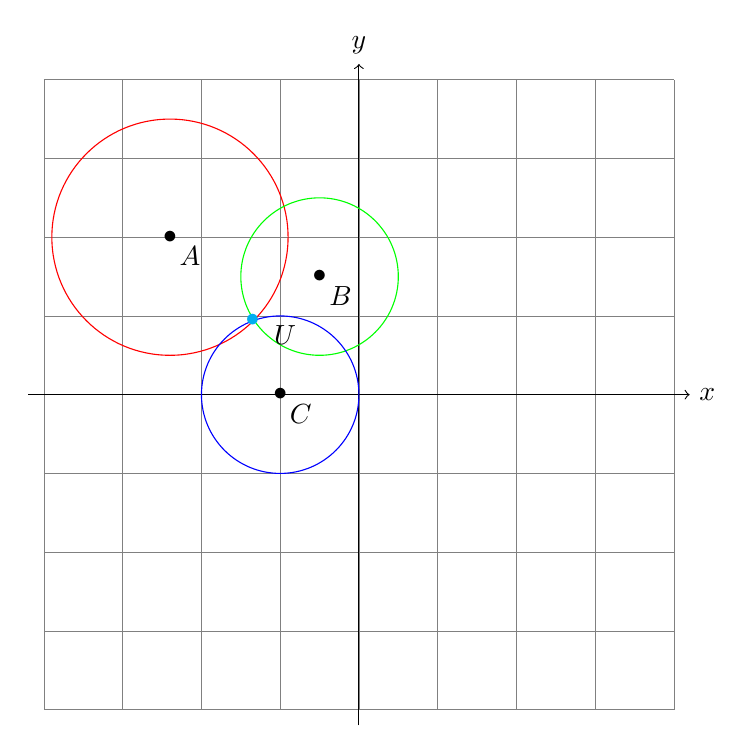
\begin{tikzpicture}
            \draw[very thin,color=gray] (-4,-4) grid (4,4);
            \draw[->] (-4.2,0) -- (4.2,0) node[right] {$x$};
            \draw[->] (0,-4.2) -- (0,4.2) node[above] {$y$};
    
            \draw[color=red] (-2.4,2) circle (1.5);
            \draw (-2.4,2) node {$\bullet$};
            \node[anchor=north west] at (-2.4,2) {$A$};
        
            \draw[color=green] (-0.5,1.5) circle (1);
            \draw (-0.5,1.5) node {$\bullet$};
            \node[anchor=north west] at (-0.5,1.5) {$B$};
        
            \draw[color=blue] (-1,0) circle (1); %2-2sqrt(3)
            \draw (-1,0) node {$\bullet$};
            \node[anchor=north west] at (-1,0) {$C$};
        
            \draw (-1.35,0.95) [cyan] node {$\bullet$};
            \node[anchor=north west] at (-1.2,1) {$U$};   
        \end{tikzpicture}
    }
    %\includegraphics{}
    \caption{}
    \label{fig:trilOK}
\end{figure}
When we step into reality however the disturbances of the signal inevitably lead to wrong estimation of the distance between the current node and the unknown node, causing the circles to intersect in wrong points or to not intersect at all, as in fig. \ref{fig:trilKO}.
\begin{figure}
    \centering
    \scalebox{1}{
        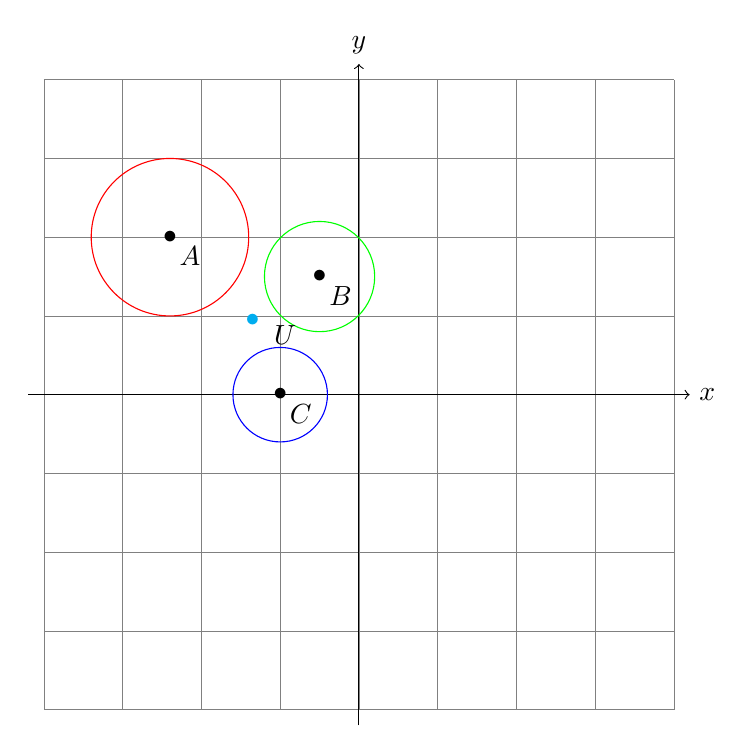
\begin{tikzpicture}
            \draw[very thin,color=gray] (-4,-4) grid (4,4);
            \draw[->] (-4.2,0) -- (4.2,0) node[right] {$x$};
            \draw[->] (0,-4.2) -- (0,4.2) node[above] {$y$};
    
            \draw[color=red] (-2.4,2) circle (1);
            \draw (-2.4,2) node {$\bullet$};
            \node[anchor=north west] at (-2.4,2) {$A$};
        
            \draw[color=green] (-0.5,1.5) circle (0.7);
            \draw (-0.5,1.5) node {$\bullet$};
            \node[anchor=north west] at (-0.5,1.5) {$B$};
        
            \draw[color=blue] (-1,0) circle (0.6); %2-2sqrt(3)
            \draw (-1,0) node {$\bullet$};
            \node[anchor=north west] at (-1,0) {$C$};
            
            \draw (-1.35,0.95) [cyan] node {$\bullet$};
            \node[anchor=north west] at (-1.2,1) {$U$};
        \end{tikzpicture}
    }
    %\includegraphics{}
    \caption{}
    \label{fig:trilKO}
\end{figure}
In the latter case, provided the algorithm has no software-level exception-catching, it would cause a runtime error, and give no results at all. However some improvements can be applied. The most intuitive one is to consider from the rssi read not just a single value but taking the max and the min values recorded during the sampling phase, and draw an annulus of possible locations as follows:
\begin{algorithm}[H]
\SetAlgoLined
\KwResult{min, max: radii of the annulus}
 Set samples = $\emptyset$\;
 \While{samples.size() < 10}{
    samples.add(new measurement)\;
 }
 min = samples.min()\;
 max = samples.max()\;
 \caption{Obtaining the derived values}
\end{algorithm}
\noindent\\The new distances will be obtained as follows:
\begin{equation}
    d^i_{min}=10^{\frac{A-min}{10\alpha}}    
\end{equation}
\begin{equation}
    d^i_{max}=10^{\frac{A-max}{10\alpha}}    
\end{equation}
The result is now given as an area that corresponds to the intersection of all the three annulus, shown in fig \ref{fig:annulus}
\begin{figure}
    \centering
    \scalebox{1.3}{
        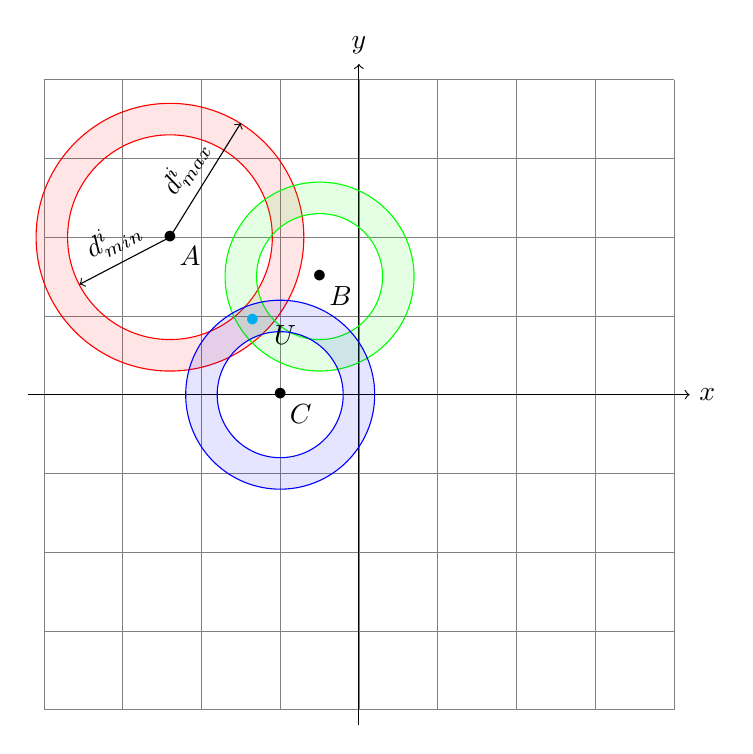
\begin{tikzpicture}
            \draw[very thin,color=gray] (-4,-4) grid (4,4);
            \draw[->] (-4.2,0) -- (4.2,0) node[right] {$x$};
            \draw[->] (0,-4.2) -- (0,4.2) node[above] {$y$};
    
            \draw[color=red] (-2.4,2) circle (1.5+0.2);
            \draw[color=red] (-2.4,2) circle (1.5-0.2);
            \fill [red,even odd rule,opacity=0.1] (-2.4,2) circle[radius=1.5+0.2] circle[radius=1.5-0.2];
            \draw[->](-2.4,2) -- (-1.5,3.45) node[midway,above,sloped] {$d^i_{max}$};
            \draw[->](-2.4,2) -- (-3.55,1.4) node[midway,above,sloped] {$d^i_{min}$};
            \draw (-2.4,2) node {$\bullet$};
            \node[anchor=north west] at (-2.4,2) {$A$};
        
            \draw[color=green] (-0.5,1.5) circle (1+0.2);
            \draw[color=green] (-0.5,1.5) circle (1-0.2);
            \fill [green,even odd rule,opacity=0.1] (-0.5,1.5) circle[radius=1+0.2] circle[radius=1-0.2];
            \draw (-0.5,1.5) node {$\bullet$};
            \node[anchor=north west] at (-0.5,1.5) {$B$};
        
            \draw[color=blue] (-1,0) circle (1+0.2); %2-2sqrt(3)
            \draw[color=blue] (-1,0) circle (1-0.2);
            \fill [blue,even odd rule,opacity=0.1] (-1,0) circle[radius=1+0.2] circle[radius=1-0.2];
            \draw (-1,0) node {$\bullet$};
            \node[anchor=north west] at (-1,0) {$C$};
            
            \draw (-1.35,0.95) [cyan] node {$\bullet$};
            \node[anchor=north west] at (-1.2,1) {$U$};
        \end{tikzpicture}
    }
    %\includegraphics{}
    \caption{}
    \label{fig:annulus}
\end{figure}
One important drawback is the low number of measurements exploited. Clearly, a higher number of samples implies a lower influence of the noise on the final estimation.
\clearpage

\section{151}
  \begin{center}
  \textbf{Assume to know:}
  \begin{itemize}
    \centering
    \item $A$
    \item $\alpha$
  \end{itemize}
  \end{center}
Consider the previous framework. As usual one can deduce the distance of the unknown node, by reverting the propagation model as done in the previous section. Then we can obtain a number of circumferences, one for each anchor node, that represent the possible locations of the unknown node. In this algorithm however you need to consider not circles but squares. The case with three anchor node can be reviewed in \cite{inproceedings}, here it is presented a logical generalization of that method with multiple nodes. More precisely, each anchor node $i$ with estimated distance $d_i$ from $n_u$ is associated to a square centered in $(x_i,y_i)$ with side equal to $2d_i$. At this point, one has a set of overlapping squares, and can easily find the intersection of all those squares,  which results in a rectangles of vertices $(x_{min},x_{max},y_{min},y_{max})$ with the following equations:
\begin{equation}
    x_{min}=\max(x_1-d_1,...,x_n-d_n)
\end{equation}
\begin{equation}
    x_{max}=\min(x_1+d_1,...,x_n+d_n)
\end{equation}
\begin{equation}
    y_{min}=\max(y_1-d_1,...,y_n-d_n)
\end{equation}
\begin{equation}
    y_{max}=\min(y_1+d_1,...,y_n+d_n)
\end{equation}
The final location will be estimated as the center of this rectangle, as follows:
\begin{equation}
    x_t=\frac{x_{min}+x_{max}}{2}
\end{equation}
\begin{equation}
    y_t=\frac{y_{min}+y_{max}}{2}
\end{equation}
The gray area in \ref{fig:mmax} shows the intersection of all the squares. The estimated point will be obtained as the center of this rectangle.
\begin{figure}
    \centering
    \scalebox{1.3}{
        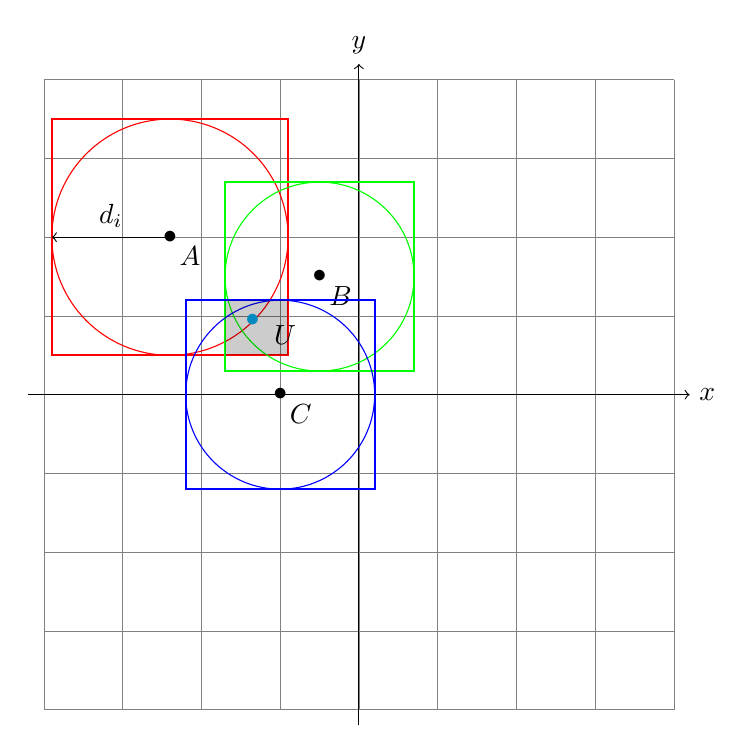
\begin{tikzpicture}
            \draw[very thin,color=gray] (-4,-4) grid (4,4);
            \draw[->] (-4.2,0) -- (4.2,0) node[right] {$x$};
            \draw[->] (0,-4.2) -- (0,4.2) node[above] {$y$};
    
            \draw[color=red] (-2.4,2) circle (1.5);
            \draw[red, thick] (-3.9,0.5) rectangle (-0.9,3.5);
            \draw[->](-2.4,2) -- (-3.9,2) node[midway,above,sloped] {$d_i$};
            \draw (-2.4,2) node {$\bullet$};
            \node[anchor=north west] at (-2.4,2) {$A$};
        
            \draw[color=green] (-0.5,1.5) circle (1.2);
            \draw[green, thick] (-1.7,0.3) rectangle (0.7,2.7);
            \draw (-0.5,1.5) node {$\bullet$};
            \node[anchor=north west] at (-0.5,1.5) {$B$};
        
            \draw[color=blue] (-1,0) circle (1.2); %2-2sqrt(3)
            \draw[blue, thick] (-2.2,-1.2) rectangle (0.2,1.2);
            \draw (-1,0) node {$\bullet$};
            \node[anchor=north west] at (-1,0) {$C$};
            
            \draw (-1.35,0.95) [cyan] node {$\bullet$};
            \node[anchor=north west] at (-1.2,1) {$U$};
            
            \fill [opacity=0.2] (-0.9,1.2) rectangle (-1.7,0.5);
        \end{tikzpicture}
    }
    %\includegraphics{}
    \caption{}
    \label{fig:mmax}
\end{figure}
does it always converge? $x_max$ is always greater than $x_min$?
\clearpage

\section{881}
  \begin{center}
  \textbf{Assume to know:}
  \begin{itemize}
    \centering
    \item $A$
    \item $\alpha$
    \item $\xi_i,\forall i$
  \end{itemize}
  \end{center}
In \cite{10.5555/2161958} you can find this version but using a slighty different model.
Consider the model ?? below reported
\begin{equation}
    \nu_i=-\beta\ln(d_i)+\xi_i
\end{equation}
After some time, for each anchor node we will have a list of measurements, drawn from the random variable 
\begin{equation}
N_i=-\beta\ln(d_i)+\xi_i.
\end{equation}
Cite ross also here, only for $\mathcal{N}+a$, and remind $xi_i\sim\mathcal{N}(0,\sigma^2_i)$. To give an idea, each anchor node outputs data as a gaussian distribution shifted by the mean, so for the anchor node we have samples extracted from $\mathcal{N}(-\beta\ln(d_i), \sigma_i^2)$. Note that $\sigma_i$ is not necessarily contant, for all $i$.

Rewrite the ?? as follows 
\begin{equation}
    \nu_i=-\ln\big(d_i^{2\frac{\beta}{2}}\big)+\xi_i
\end{equation}
By exponentiating both members of ??(previous) we have 
\begin{equation}
    e^{\nu_i}=e^{-\ln\big(d_i^{2\frac{\beta}{2}}\big)+\xi_i}
\end{equation}
\begin{equation}
    \bigg(e^{\nu_i}\bigg)^{-1}=\bigg(e^{-\ln\big(d_i^{2\frac{\beta}{2}}\big)+\xi_i}\bigg)^{-1}
\end{equation}
\begin{equation}
    e^{-\nu_i}=e^{\ln\big(d_i^{2\frac{\beta}{2}}\big)-\xi_i}
\end{equation}
\begin{equation}
    e^{-\nu_i}=d_i^{2\frac{\beta}{2}}e^{-\xi_i}
\end{equation}
\begin{equation}
    \bigg(e^{-\nu_i}\bigg)^{\frac{2}{\beta}}=\bigg(d_i^{2\frac{\beta}{2}}e^{-\xi_i}\bigg)^{\frac{2}{\beta}}
\end{equation}
\begin{equation}
    e^{-\frac{2}{\beta}\nu_i}=d_i^2e^{-\frac{2}{\beta}\xi_i}
\end{equation}
Remind that $\xi_i\sim \mathcal{N}(0,\sigma^2_i)$ is a zero-mean gaussian distribution. The exponentiation of a gaussian distribution is \cite{Beran2011} a log-normal distribution. In other words, given $X\sim \mathcal{N}(\mu,\sigma^2)$, then $Y=e^X\sim \text{Lognormal}(\mu,\sigma^2)$ with
\begin{equation}
    E[Y]=E\big[e^X\big]=e^{\mu+\frac{\sigma^2}{2}}
\end{equation}
\begin{equation}
    Var[Y]=Var\big[e^X\big]=(e^{\sigma^2}-1)e^{2\mu+\sigma^2}
\end{equation}
From \cite{alma9926534668905776}, it is clear that if $a\in \mathbb{R}$ and $X\sim \mathcal{N}(\mu,\sigma^2)$ then
\begin{equation}
aX\sim \mathcal{N}(a\mu,a^2\sigma^2)    
\end{equation}
so in this case, 
\begin{equation}
    -\frac{2}{\beta}\xi_i\sim \mathcal{N}\bigg(0,\frac{4}{\beta^2}\sigma^2_i\bigg)
\end{equation}
From equations ?? and ?? (previous equation)
\begin{align}
    &E\bigg[e^{-\frac{2}{\beta}\nu_i}\bigg]\\
    &=E\bigg[d_i^2e^{-\frac{2}{\beta}\xi_i}\bigg]\\
    &=d_i^2E\bigg[e^{-\frac{2}{\beta}\xi_i}\bigg]\\ &=d_i^2e^{\frac{2}{\beta^2}\sigma^2_i}
\end{align}
\begin{align}
    &Var\bigg[e^{-\frac{2}{\beta}\nu_i}\bigg]\\
    &=Var\bigg[d_i^2e^{-\frac{2}{\beta}\xi_i}\bigg]\\
    &=d_i^4Var\bigg[e^{-\frac{2}{\beta}\xi_i}\bigg]\\
    &=d_i^4(e^{\frac{4}{\beta^2}\sigma_i^2}-1)e^{\frac{4}{\beta^2}\sigma^2_i}
\end{align}
As we can see from ??, $e^{-\frac{2}{\beta}\nu_i}$ is a biased estimate of $d_i^2$ since from ?? its mean is not $d_i^2$ as we wanted, however we can remove its bias by dividing it by $e^{\frac{2}{\beta^2}\sigma^2_i}$. Therefore, an unbiased estimate of $d_i^2$ is 
\begin{equation}
    e^{-\frac{2}{\beta}\nu_i-\frac{2}{\beta^2}\sigma^2_i}
\end{equation}
We want to use the above estimator obtained from the measurements to build a linear models in $\mathbf{x}$. Since the estimator is now unbiased by writing 
\begin{equation}
    d_i^2=(x-x_i)^2+(y-y_i)^2
\end{equation}
we can write
\begin{equation}
    (x-x_i)^2+(y-y_i)^2=e^{-\frac{2}{\beta}\nu_i-\frac{2}{\beta^2}\sigma^2_i}
\end{equation}
\begin{equation}
    -2x_ix-2y_iy+x^2+y^2+x_i^2+y_i^2=e^{-\frac{2}{\beta}\nu_i-\frac{2}{\beta^2}\sigma^2_i}
\end{equation}
\begin{equation}
    -2x_ix-2y_iy+x^2+y^2=e^{-\frac{2}{\beta}\nu_i-\frac{2}{\beta^2}\sigma^2_i}-x_i^2-y_i^2
\end{equation}
By calling $R^2=x^2+y^2$ we can write it in matrix form
\begin{equation}
    \begin{bmatrix}
        -2x_1 & -2y_1 & 1\\
        \vdots&\vdots&\vdots\\
        -2x_n & -2y_n & 1
    \end{bmatrix}
    \begin{bmatrix}
        x\\
        y\\
        R^2
    \end{bmatrix} = 
    \begin{bmatrix}
       e^{-\frac{2}{\beta}\nu_1-\frac{2}{\beta^2}\sigma^2_1} & -x_1^2 & -y_1^2\\
        \vdots&\vdots&\vdots\\
        e^{-\frac{2}{\beta}\nu_n-\frac{2}{\beta^2}\sigma^2_n} & -x_n^2 & -y_n^2\\
    \end{bmatrix}
\end{equation}
with $$M=\begin{bmatrix}
        -2x_1 & -2y_1 & 1\\
        \vdots&\vdots&\vdots\\
        -2x_n & -2y_n & 1
    \end{bmatrix}$$
$$\theta^* =     \begin{bmatrix}
        x\\
        y\\
        R^2
    \end{bmatrix}$$
$$b=    \begin{bmatrix}
        e^{-\frac{2}{\beta}\nu_1-\frac{2}{\beta^2}\sigma^2_1} & -x_1^2 & -y_1^2\\
        \vdots&\vdots&\vdots\\
        e^{-\frac{2}{\beta}\nu_n-\frac{2}{\beta^2}\sigma^2_n} & -x_n^2 & -y_n^2\\
    \end{bmatrix}$$
Now since $\theta^*$ is unknown we would like to choose $\theta\approx\theta^*$ to have 
\begin{equation}
    M\theta-b\approx0
\end{equation}
One easy way is to seek the minimum of 
\begin{equation}
    J(\theta)=(M\theta - b)^T(M\theta - b)
\end{equation}
We can fit this model with the Least Square Method, that for a linear model (which is the ours) has a known explicit solution \cite{10.5555/1557273,}:
\begin{equation}
    \hat{\theta}=(M^TM)^{-1}M^Tb
\end{equation}
the target position can be finally obtained as 
\begin{equation}
\begin{bmatrix}
    \hat{x}\\
    \hat{y}
\end{bmatrix}=
\begin{bmatrix}
    [\hat{\theta}]_1\\
    [\hat{\theta}]_2
\end{bmatrix}
\end{equation}
\clearpage


\section{270}
As we have seen in the case before we have used the statistics, to obtain an estimator for a given distibution. However we can still improve it by giving to each anchor node a weight, bound to the variance of the anchor node itself, in a way to give more importance to the nodes that produces a steadier output (low variance) and less importance to those nodes that produces more irregular values (high variance). To ease the computation we consider each anchor node to be independent from each other. It is important to note that this improvement affects only the LLS computation, and not the definition of the estimator. The choice of the symmetric weighting matrix $W$ will be done according to BLUE (Best Linear Unbiased Estimator) \cite{899498y4hd,10.5555/151045}.
The new cost function will be
\begin{equation}
    J(\theta)=(M\theta-b)^TW(M\theta-b)
\end{equation}
Following the LLS framework,
\begin{equation}
    \hat{\theta}=\arg \min_{\theta} J(\theta)=(\mathbf{M}^T\mathbf{WM})^{-1}\mathbf{M^TWb}
\end{equation}
rewrite better\\\\
So we need to compute the variance of each estimator $\hat{d_i^2}$, correct the hat also in the previous

\begin{align}
&Var\big[\hat{d_i^2}\big]=&& \text{comment example } x\\
&=Var\bigg[e^{-\frac{2}{\beta}\nu_i-\frac{2}{\beta^2}\sigma^2_i}\bigg]\\
&=\bigg(e^{-\frac{2}{\beta^2}\sigma^2_i}\bigg)^2Var\bigg[e^{-\frac{2}{\beta}\nu_i}\bigg]\\
&=\cancel{e^{-\frac{4}{\beta^2}\sigma^2_i}}d_i^4\bigg(e^{\frac{4}{\beta^2}\sigma_i^2}-1\bigg)\cancel{e^{\frac{4}{\beta^2}\sigma^2}}\\
&=d_i^4\bigg(e^{\frac{4}{\beta^2}\sigma_i^2}-1\bigg)\\
&\approx \big(\hat{d_i}^2\big)^2\bigg(e^{\frac{4}{\beta^2}\sigma_i^2}-1\bigg)\\
&=\bigg(e^{-\frac{2}{\beta}\nu_i-\frac{2}{\beta^2}\sigma^2_i}\bigg)^2\bigg(e^{\frac{4}{\beta^2}\sigma_i^2}-1\bigg)\\
&=e^{-\frac{4}{\beta}\nu_i-\frac{4}{\beta^2}\sigma^2_i}\bigg(e^{\frac{4}{\beta^2}\sigma^2_i}-1\bigg)\\
&=e^{-\frac{4}{\beta}\nu_i}\bigg(1-e^{-\frac{4}{\beta^2}\sigma^2_i}\bigg)\\
&=\frac{1-e^{-\frac{4}{\beta^2}\sigma^2_i}}{e^{\frac{4}{\beta}\nu_i}}
\end{align}
Therefore, the estimate is given with the improved equation ?? and the optimum weight matrix \cite{5765553} is 
\begin{align}
    &\mathbf{W}=\text{diag}\big((\sigma^2_{d_1})^{-1},...,(\sigma^2_{d_n})^{-1}\big)\\
    &=\text{diag}\bigg(\frac{e^{\frac{4}{\beta}\nu_1}}{1-e^{-\frac{4}{\beta^2}\sigma^2_1}},...,\frac{e^{\frac{4}{\beta}\nu_n}}{1-e^{-\frac{4}{\beta^2}\sigma^2_n}}\bigg)
\end{align}
\clearpage

\subsection{510}
  \begin{center}
  \textbf{Assume to know:}
  \begin{itemize}
    \centering
    \item $A$
    \item $\alpha$
  \end{itemize}
  \end{center}
From the canonical model extract $d_i$ as follows
\begin{equation*}
    10^{RSSI_{i}}=10^{A-\alpha\log_{10}(d_i)}
\end{equation*}
\begin{equation*}
    10^{RSSI_{i}-A}=10^{-\alpha\log_{10}(d_i)}
\end{equation*}
\begin{equation*}
     10^{RSSI_{i}-A}=d_i^{-\alpha}
\end{equation*}
\begin{equation}
    d_i=10^{\frac{A-RSSI_{i}}{\alpha}}
\end{equation}
so that we have the following set of equations
\begin{align}
\begin{split} 
(x_1-x)^2+(y_1-y)^2&=d_1^2 \\ 
(x_2-x)^2+(y_2-y)^2&=d_2^2 \\ 
&\;\;\vdots\\
(x_n-x)^2+(y_n-y)^2&=d_n^2 \\
\end{split}
\end{align}
Consider 
\begin{align}
\frac{1}{n}&\sum_{i=1}^nd_i^2=\\
&=\frac{1}{n}\sum_{i=1}^n\big[(x_i-x)^2+(y_i-y)^2\big]\\
&=\frac{1}{n}\sum_{i=1}^n(x_i-x)^2+\frac{1}{n}\sum_{i=1}^n(y_i-y)^2\\
&=\frac{1}{n}\sum_{i=1}^n[x_i^2-2x_ix+x^2] + \frac{1}{n}\sum_{i=1}^n[y_i^2-2y_iy+y^2]\\
&=\frac{1}{n}\sum_{i=1}^n[x_i^2]-2x\frac{1}{n}\sum_{i=1}^n[x_i]+ x^2 + \frac{1}{n}\sum_{i=1}^n[y_i^2]-2y\frac{1}{n}\sum_{i=1}^n[y_i]+ y^2
\end{align}
Frone one of the ?? it follows
\begin{equation}
x_i^2+x^2-2x_ix+y_i^2+y^2-2y_iy=d_i^2      
\end{equation}
\begin{equation}
-x_i^2-x^2+2x_ix-y_i^2-y^2+2y_iy=-d_i^2      
\end{equation}
Now by adding ?? to ?? previous you have 
\begin{equation}
\begin{split}
    \bigg(-x_i^2  + \frac{1}{n}\sum_{i=1}^n[x_i^2]\bigg)+
    \bigg(-y_i^2+ \frac{1}{n}\sum_{i=1}^n[y_i^2]\bigg)+\\
    +\bigg(2x_ix-2x\frac{1}{n}\sum_{i=1}^n[x_i]\bigg)+
    \bigg(2y_iy -2y\frac{1}{n}\sum_{i=1}^n[y_i]\bigg)
    =\frac{1}{n}&\sum_{i=1}^n[d_i^2]-d_i^2
\end{split}    
\end{equation}
and by rearranging the equation
\begin{equation}
\begin{split}
    +2x\bigg(x_i-\frac{1}{n}\sum_{i=1}^n[x_i]\bigg)+
    2y\bigg(y_i -\frac{1}{n}\sum_{i=1}^n[y_i]\bigg)\\
    \bigg(-x_i^2  + \frac{1}{n}\sum_{i=1}^n[x_i^2]\bigg)+
    \bigg(-y_i^2+ \frac{1}{n}\sum_{i=1}^n[y_i^2]\bigg)+
    =\frac{1}{n}&\sum_{i=1}^n[d_i^2]-d_i^2
\end{split}    
\end{equation}
then the previous set of equations ?? becomes
\begin{align}
\begin{split} 
    \bigg(x_1-\frac{1}{n}&\sum_{i=1}^nx_i\bigg)x+\bigg(y_1-\frac{1}{n}\sum_{i=1}^ny_i\bigg)y\\
    &=\frac{1}{2}\bigg[\bigg(x_1^2-\frac{1}{n}\sum_{i=1}^nx^2_i\bigg)+\bigg(y_1^2-\frac{1}{n}\sum_{i=1}^ny^2_i\bigg)-\bigg(d_1^2-\frac{1}{n}\sum_{i=1}^nd_i^2\bigg)\bigg]\\
&\;\;\vdots\\
    \bigg(x_n-\frac{1}{n}&\sum_{i=1}^nx_i\bigg)x+\bigg(y_n-\frac{1}{n}\sum_{i=1}^ny_i\bigg)y\\
    &=\frac{1}{2}\bigg[\bigg(x_n^2-\frac{1}{n}\sum_{i=1}^nx^2_i\bigg)+\bigg(y_n^2-\frac{1}{n}\sum_{i=1}^ny^2_i\bigg)-\bigg(d_n^2-\frac{1}{n}\sum_{i=1}^nd_i^2\bigg)\bigg]
\end{split}
\end{align}
So can write the above set of equations in matricial form $\mathbf{Mx}=\mathbf{b}$ by setting
$$
\mathbf{M}=\begin{bmatrix}
    x_1-\frac{1}{n}\sum_{i=1}^nx_i&y_1-\frac{1}{n}\sum_{i=1}^ny_i\\
    \vdots&\vdots\\
    x_n-\frac{1}{n}\sum_{i=1}^nx_i&y_n-\frac{1}{n}\sum_{i=1}^ny_i
\end{bmatrix}
$$
$$
\mathbf{x}=\begin{bmatrix}
    x\\
    y
\end{bmatrix}
$$
$$\mathbf{b}=\frac{1}{2}
\begin{bmatrix}
\bigg(x_1^2-\frac{1}{n}\sum_{i=1}^nx^2_i\bigg)+\bigg(y_i^2-\frac{1}{n}\sum_{i=1}^ny^2_i\bigg)-\bigg(d_i^2-\frac{1}{n}\sum_{i=1}^nd_i^2\bigg)\\
\vdots\\
\bigg(x_n^2-\frac{1}{n}\sum_{i=1}^nx^2_i\bigg)+\bigg(y_n^2-\frac{1}{n}\sum_{i=1}^ny^2_i\bigg)-\bigg(d_n^2-\frac{1}{n}\sum_{i=1}^nd_i^2\bigg)
\end{bmatrix}
$$
then the solution can be computed with the usual Linear Least Square procedure obtaining
\begin{equation}
    \mathbf{x}=(\mathbf{M^TM})^{-1}\mathbf{M^Tb}
\end{equation}
Also valid for non RSSI based localization
\clearpage


\section{858}
Let's start from a geometrical analysis. Given two intersecting circles at center $x_{1},y_{1}$ and $x_{2},y_{2}$ respectively and with radius $r_1$ and $r_2$ respectively, the line that passes by the two points of intersection has the following equation
\begin{equation}
    (x_2-x_1)x+(y_2-y_1)y=\frac{1}{2}\big[(x_2^2+y_2^2)-(x_1^2+y_1^2)-(r_2^2-r_1^2)\big]
\end{equation}
from subtracting one equation of the circle to the other. Now a question arise, given the noise effect on the measurements, what happens if the two circles are not intersecting? Is the formula still valid? Yes. Why?... 

The formula can be obtained by deriving $m$ and $q$. The parameter $m$ in the perpendicular to line passing between the two centers.

Given $n$ measurements (so $n$ circles), only $n-1$ are needed to have an independent system of equations. For example, for the trilateration method, (thus with three circles), it is needed to have only 2 lines, for example the line passing between the first and the second circle, and the line passing between the first and the third one. (optimization! given instead using only the first circle use the previous one: (1,2), (1,3) use (1,2), (2,3)).
Therefore, given $n$ points we have a set of $n-1$ equations like the above ??, that can be written in matricial form $\mathbf{Mx}=\mathbf{b}$ with
$$\mathbf{M}=\begin{bmatrix}
x_2-x_1&y_2-y_1\\
x_3-x_1&y_3-y_1\\
\vdots&\vdots\\
x_n-x_1&y_n-y_1
\end{bmatrix}$$
$$\mathbf{x}=\begin{bmatrix}
x\\
y
\end{bmatrix}$$
$$\mathbf{b}=\begin{bmatrix}
(x^2_2+y^2_2)-(x_1^2+y^2_1)-(d_2^2-d_1^2)\\
(x^2_3+y^2_3)-(x_1^2+y^2_1)-(d_3^2-d_1^2)\\
\vdots\\
(x^2_n+y^2_n)-(x_1^2+y^2_1)-(d_n^2-d_1^2)\\
\end{bmatrix}$$
The solution is obtained as an approximated intersection of all these lines with the LLS.

Given the high influence in this formula of the first anchor node (present in all equations), one can try an optimization by rearranging the above formula in a way that it relays more evenly to the all nodes as follows
$$\mathbf{M}=\begin{bmatrix}
x_2-x_1&y_2-y_1\\
x_3-x_2&y_3-y_2\\
\vdots&\vdots\\
x_n-x_{n-1}&y_n-y_{n-1}
\end{bmatrix}$$
$$\mathbf{x}=\begin{bmatrix}
x\\
y
\end{bmatrix}$$
$$\mathbf{b}=\begin{bmatrix}
(x^2_2+y^2_2)-(x_1^2+y^2_1)-(d_2^2-d_1^2)\\
(x^2_3+y^2_3)-(x_2^2+y^2_2)-(d_3^2-d_2^2)\\
\vdots\\
(x^2_n+y^2_n)-(x_{n-1}^2+y^2_{n-1})-(d_n^2-d_{n-1}^2)\\
\end{bmatrix}$$
Highly resistant to noise. Always gives a result. Fast.
\clearpage


\section{435}
If you assume to know $A$ then good results with GN method...\\
This algorithm is the generalization of the trilateration method, and is known as multilateration. 
This method can provide two main benefits over the classic trilateration:
\begin{itemize}
    \item Always exists a solution (the algorithm may not be able to find it though)
    \item The result is made on more observation than the trilateration
\end{itemize}
The first point can be explained as follows:
We start by measuring the rssi value in each position.This measurement can be fitted to the model of $RSSI$ propagation. Assuming that the exact distribution follows 
\begin{equation}
rssi(x,y)=A^*-10\alpha^*\log_{10}\big(\sqrt{(x_t^*-x)^2+(y_t^*-y)^2}\big)    
\end{equation}
with $A^*,\alpha^*,x^*_t,y^*_t$ unknown, we can write a performance index $J$
\begin{equation}
    J(A,n,x_t,y_t)=\sum_{i=1}^n\bigg(rssi_i-A+10\alpha\log_{10}\big(\sqrt{(x_i-x_t)^2+(y_i-y_t)^2}\big)\bigg)
\end{equation}
and then choosing 
\begin{equation}
\Bar{x_t}, \Bar{y_t}=\arg \min_{A,\alpha,x_t,y_t}J(A,\alpha,x_t,y_t)
\end{equation}
\clearpage


\section{486}
When the error follows a zero mean gaussian distribution, this method is a weighted version of the Nonlinear Multilateration method. 
\begin{equation}
    \beta=\frac{\alpha}{\ln(10)}
\end{equation}
Each anchor $i$ has a distribution like $\mathcal{N}(-\beta\ln(d_i),\sigma^2_i)$
A look more closely related to the probability point of view is
\begin{equation}
    \pi(\nu_i)=\frac{1}{\sqrt{2\pi\sigma^2_{\nu_i}}}e^{-\frac{1}{2}\frac{(\nu_i+\alpha\ln(d_i))^2}{\sigma^2_{\nu_i}}}
\end{equation}
$\mathbf{\Sigma}$ is diagonal for uncorrelated (remember independent implies uncorrelated, but not the reverse) variables
$$\mathbf{f}(\mathbf{x})=-\beta\begin{bmatrix}
\ln(\sqrt{(x-x_1)^2+(y-y_1)^2})\\
\vdots\\
\ln(\sqrt{(x-x_n)^2+(y-y_n)^2})
\end{bmatrix}$$
For $n$ indepentent and (identically? mean is the value read which changes) distributed, the joint probabilty distribution is the product
\begin{equation}
    \pi(\mathbf{RSS})=\frac{1}{(2\pi)^{\frac{n}{2}}\Pi_{i=1}^n\sigma_{\nu_i}}e^{-\frac{1}{2}\sum_{i=1}^n\frac{(\nu_i+\alpha\ln(d_i))^2}{\sigma^2_{\nu_i}}}
\end{equation}
\begin{equation}
    \pi(\mathbf{r}_{RSS})=\frac{1}{(2\pi)^{\frac{n}{2}}|\mathbf{\Sigma}|^{\frac{1}{2}}}e^{-\frac{1}{2}\big(\mathbf{r}_{RSS}-\mathbf{f}(\mathbf{x})\big)\mathbf{\Sigma}^{-1}\big(\mathbf{r}_{RSS}-\mathbf{f}(\mathbf{x})\big)}
\end{equation}
For the Maximum Likelihood method we need to find the minimum of ??. To facilitate it we consider the log. The first part is independent of x, so we need only to maxmize the second part. We can now remove the logarithm because it is a monotonic increasing function, then we oibtain the previous forumula to be minimized. As you can see when $\mathbf{\Sigma}=diag{(\sigma_1,...)}$. The solution can be found with Newton raphson, GN...


From \cite{KAUR201982} and also each bibliography
\clearpage


\section{Centroid algorithm 677}
The algorithm works in two phases: the first phase is that each node bradcast its location to all the nearby device with RSSI above the threshold (a computed RSSI value). After that each node compute the centroid as average of all the position received. Low accuracy, may be difficult to determine threshold value. many unknown nodes, depends on the physical location of the anchor nodes, assume some regularity.
\section{Weighted centroid algorithm 306}
just use $w_{u,i}=\frac{1}{h_{u,i}}$ h is hop count, then centroid is weighted, not simple average


\section{little improvement IWCL 117}
$\bigg(\frac{1}{h_{u,i}}\bigg)^{\frac{r}{k}}$
where k is the average of all hop size


\section{EWCL 777}
from article cited, also results
\clearpage

\section{DV-Hop Algorithm 422}
Three phases. First: each anchor node sends a packet, its GPS location and hop count initially set to 0. Then the nodes that receive the packets sends it to its neigboring nodes by increasing its hop count by one. Every packet extract the minimum hop count and position information of each other node. then average hop distance (physical distance between al nodes/number of hops...), the multiplies this to the numerb of hops and get a estimate of the distance from the unknown node to each node. Then (little different from the previous?) LLS is used.
\clearpage


\section{Fingerprinting 437}
from \cite{YIU2017235} 1-NN compares how each anchor node sees all the other nodes to how the unknown node reads the rssi of all the anchor nodes. Then the estimated location would be the anchor node closest to the unknown node. kNN takes the mean of the first k 






\chapter{Conclusioni (1 pag)}









\clearpage
\printbibliography[
heading=bibintoc,
title={Whole bibliography}
]
%Prints the entire bibliography with the title "Whole bibliography"

\clearpage

%Filters bibliography
\printbibliography[heading=subbibintoc,type=article,title={Articles only}]
%\printbibliography[type=book,title={Books only}]
%\printbibliography[keyword={physics},title={Physics-related only}]
%\printbibliography[keyword={latex},title={\LaTeX-related only}]

\end{document}
